\documentclass[10pt,a4paper]{article}
\usepackage[margin=0.5in]{geometry}
\usepackage{tikz}
\usepackage{amsmath}
\usepackage{pgfplots}
\usepackage{gensymb}
\usepackage{pgf-pie}  

\begin{document}

\title{Year 5 Mathematics Examination}
\date{}
\maketitle

\section*{Arithmetic}

\begin{enumerate}
\item $563 + 231$
\item $809 - 567$
\item $14 \times 7$
\item $741 \div 27$
\item $24 \times 12$
\item $2003 - 456$
\item $534 + 198$
\item $540 \div 18$
\item $889 - 345$
\item $27 \times 8$
\end{enumerate}

\section*{Number And Place Value}

\begin{enumerate}
\setcounter{enumi}{10}
\item Write 8709 in words.
\item Write nine hundred thousand in numbers.
\item Write 50670 in words.
\item Write four thousand in numbers.
\end{enumerate}

\section*{Fractions}

\begin{enumerate}
\setcounter{enumi}{14}
\item Express $7$ as a fraction of $10$.
\item What is $\frac{4}{5}$ of 30?
\item Express $16$ as a fraction of $20$.
\item What is $\frac{2}{3}$ of 18?
\end{enumerate}

\section*{Decimals}

\begin{enumerate}
\setcounter{enumi}{18}
\item Convert 0.625 to a fraction in simplest form.
\item Add 13.6 and 1.45.
\item Convert 0.25 to a fraction in simplest form.
\item Add 1.25 and 0.75.
\end{enumerate}

\section*{Percentages}

\begin{enumerate}
\setcounter{enumi}{22}
\item Increase 250 by 15\%.
\item What is 25\% of 300?
\item Increase 400 by 25\%.
\item What is 30\% of 600?
\end{enumerate}

\section*{Measurement And Geometry}

\begin{enumerate}
\setcounter{enumi}{26}
\item Calculate the area of a rectangle with width 5 cm and length 11 cm.
\item What is the perimeter of a square with side length 13 cm?
\item Calculate the area of a rectangle with width 6 cm and length 16 cm.
\item What is the perimeter of a square with side length 8 cm?
\item Calculate the area of a triangle with base 5 cm and height 7 cm.
\item What is the perimeter of a rectangle with width 3 cm and length 10 cm?
\item Calculate the area of a triangle with base 6 cm and height 9 cm.
\end{enumerate}

\section*{Graphs and Bar Charts}

\begin{enumerate}
\setcounter{enumi}{33}
\item 
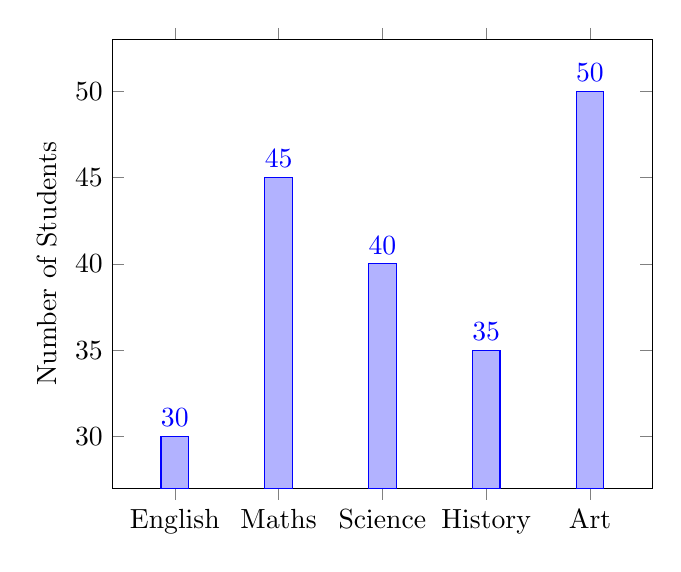
\begin{tikzpicture}
\begin{axis}[
    ybar,
    enlargelimits=0.15,
    ylabel={Number of Students},
    symbolic x coords={English,Maths,Science,History,Art},
    xtick=data,
    nodes near coords,
    nodes near coords align={vertical},
]
\addplot coordinates {(English,30) (Maths,45) (Science,40) (History,35) (Art,50)};
\end{axis}
\end{tikzpicture}

\item What subject has the most students?
\item What is the total number of students in all subjects?
\item 

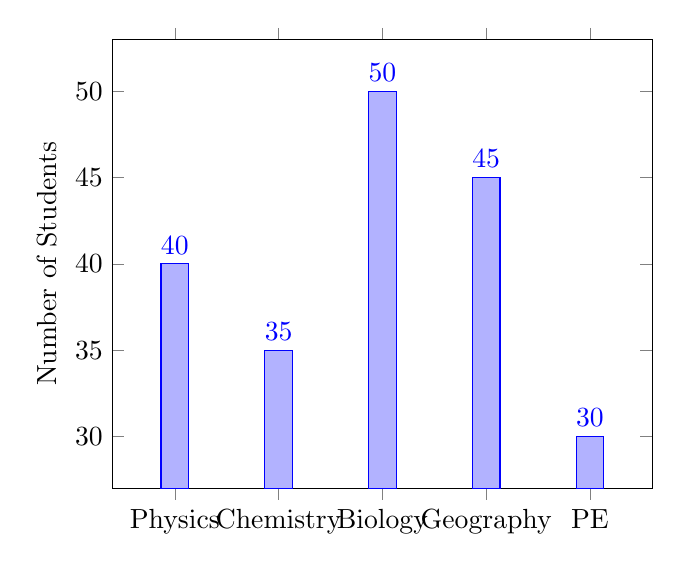
\begin{tikzpicture}
\begin{axis}[
    ybar,
    enlargelimits=0.15,
    ylabel={Number of Students},
    symbolic x coords={Physics,Chemistry,Biology,Geography,PE},
    xtick=data,
    nodes near coords,
    nodes near coords align={vertical},
]
\addplot coordinates {(Physics,40) (Chemistry,35) (Biology,50) (Geography,45) (PE,30)};
\end{axis}
\end{tikzpicture}

\item What subject has the fewest students?
\item What is the total number of students in all subjects?
\item 

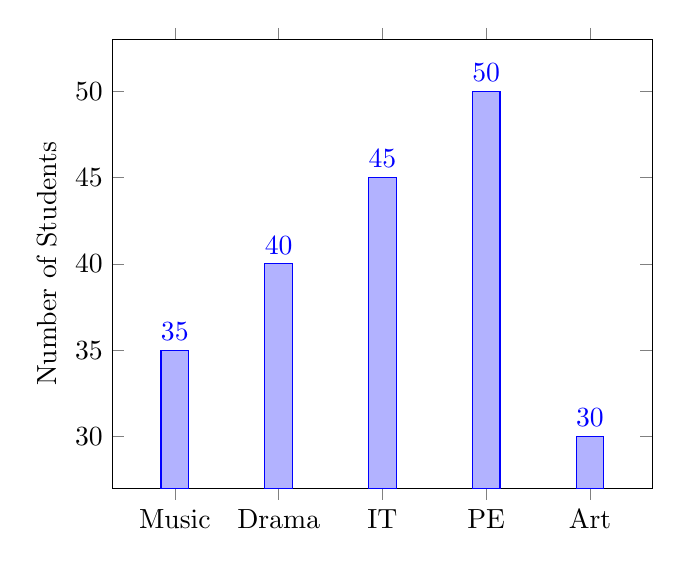
\begin{tikzpicture}
\begin{axis}[
    ybar,
    enlargelimits=0.15,
    ylabel={Number of Students},
    symbolic x coords={Music,Drama,IT,PE,Art},
    xtick=data,
    nodes near coords,
    nodes near coords align={vertical},
]
\addplot coordinates {(Music,35) (Drama,40) (IT,45) (PE,50) (Art,30)};
\end{axis}
\end{tikzpicture}

\item What subject has the most students?
\item What is the total number of students in all subjects?
\end{enumerate}

\section*{Clock and Time}

\begin{enumerate}
\setcounter{enumi}{38}
\item What time will it be 4 hours after 3:00 PM?
\item If it is now 9:00 AM, what was the time 3 hours and 15 minutes ago?
\item A movie starts at 7:30 PM and lasts for 1 hour and 45 minutes. At what time does the movie end?
\item If a train departs at 10:00 AM and arrives at 4:00 PM, how long is the train journey?
\item How many minutes are there from 3:00 PM to 5:15 PM?
\end{enumerate}

\section*{Distance}

\begin{enumerate}
\setcounter{enumi}{43}
\item If John walks at a speed of 4 km/h, how far will he travel in 3 hours?
\item Mary cycles at a speed of 12 km/h. How far does she cycle in 45 minutes?
\item If a car travels 100 km in 2 hours, what is its speed in km/h?
\item A bus travels 80 km in 4 hours. What is its speed in km/h?
\item Peter runs at a speed of 6 km/h. How long does it take him to run 18 km?
\end{enumerate}

\section*{Pie Charts}

\begin{enumerate}
\setcounter{enumi}{48}
\item
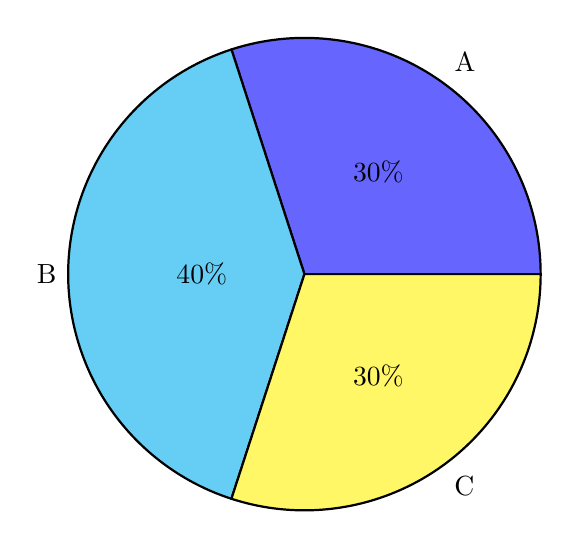
\begin{tikzpicture}
\pie{30/A, 40/B, 30/C}
\end{tikzpicture}

What percentage is category B?

\item 
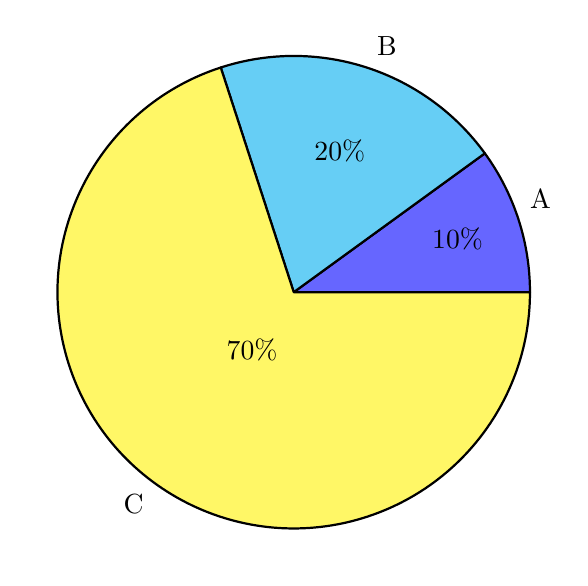
\begin{tikzpicture}
\pie{10/A, 20/B, 70/C}
\end{tikzpicture}

What percentage is category C?

\item 
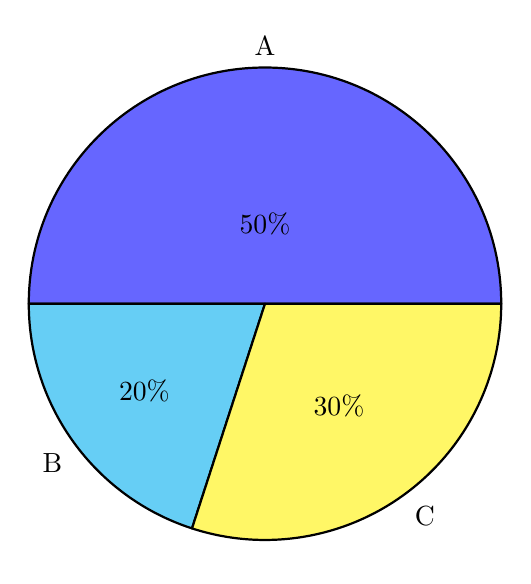
\begin{tikzpicture}
\pie{50/A, 20/B, 30/C}
\end{tikzpicture}

What percentage is category A?

\item 
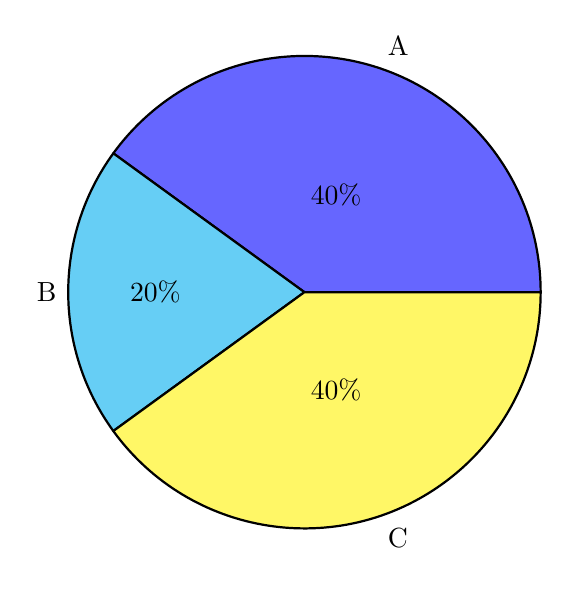
\begin{tikzpicture}
\pie{40/A, 20/B, 40/C}
\end{tikzpicture}

What percentage is category B?

\item 
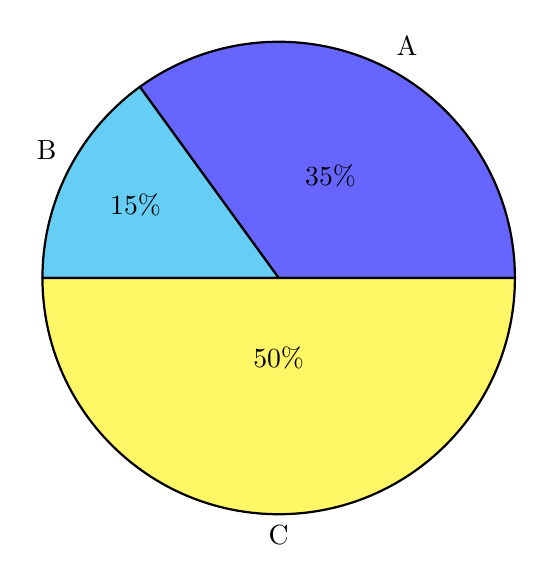
\begin{tikzpicture}
\pie{35/A, 15/B, 50/C}
\end{tikzpicture}

What percentage is category C?
\end{enumerate}

\end{document}
